\documentclass{article}
\usepackage[utf8]{inputenc}
\usepackage{enumitem}
\usepackage{amsmath}
\usepackage[normalem]{ulem}
\usepackage{eurosym}
\usepackage{amsfonts}
\usepackage{amssymb}

%PACKAGE ILLUSTRATION
\usepackage{tikz}
\usetikzlibrary{3d,calc}


\title{Cours de maths synthétique (pour \sout{X/ENS} CCINP/CENTRALE/MINES)}

\author{Crée par des gens de la PSI de Claude B}


\begin{document}

\maketitle

\newpage

\tableofcontents

\newpage

\section{Algèbre}

\subsection{Non assigné pour l'instant}
\begin{itemize}[label=$\ast$]
	\item Soit A et B deux parties de E. Si A est une partie génératrice de E et si \( A \subset B \) alors B est une parties génératrice de E (c'est la même chose pour les familles)
	\item Une symétrie s est un automorphisme donc \(s^{-1} = s \)
	\item 	\( Mat_B(v \circ u) = Mat_B(v)Mat_B(u) \)
	\item \underline{inégalité triangulaire} : \( \|a + b\| \leq \|a\| + \|b\| \)
	\item \underline{théorème de pythagore} : \( \|x + y\| = \|x\| + \|y\| \) ssi x et y sont orthogonaux
	\item Toute famille orthogonale de vecteurs non nuls de E est libre, en particulier, toute famille orthonormée de E est libre
	\item \underline{Théorème de la base orthonormée incomplète} : Toute famille orthonormée de E peut être complétée en une base orthonormée de E
	\item \underline{Théorème de la base incomplète} : Toute famille libre fini d'un EV de dimension fini peut être complété en une base de cet EV
	\item \underline{Théorème de la base extraite} : Toutes familles génératrice finie d'un EV fini on peut extraire une base de cet EV
	\item Toute espace euclidien possède une base orthonormée
	\item \textbf{Formule de Leibniz pour les polynômes :} Pour \( P, Q \in K[X] \) et \( n \in N \), alors \[ (PQ)^{(n)} = \sum_{k=0}^{n} \binom{n}{k} P^{(k)}Q^{(n-k)} \].
	\item \textbf{Formule de Taylor pour les polynômes :} Pour \( P \in K[X] \) et \( a \in K \), alors \[ P(X) = \sum_{n \geq 0} \frac{P^{(n)}(a)}{n!}(X - a)^n \].
	\item \textbf{Théorème (division euclidienne des polynômes) :} Soient \( A, B \in K[X] \) avec \( B \) non nul. Il existe un unique couple \( (Q, R) \in K[X] \) tel que \( A = BQ + R \) et \( \deg(R) < \deg(B) \).
	\item \textbf{Propriétés des matrices :} Soient \( A, B \in GL_n(K) \).
\begin{enumerate}
    \item Si \( AB \in GL_n(K) \), alors \( (AB)^{-1} = B^{-1}A^{-1} \).
    \item Si \( A^T \in GL_n(K) \), alors \( (A^T)^{-1} = (A^{-1})^T \).
\end{enumerate}

\item \textbf{Caractérisation des sous-espaces vectoriels :} Une partie \( F \) de \( E \) est un sous-espace vectoriel de \( E \) si et seulement si les trois propriétés suivantes sont vérifiées :
\begin{enumerate}
    \item \( \mathbf{0}_E \in F \) ;
    \item Pour tout \( (x, y) \in F^2 \), \( x + y \in F \) ;
    \item Pour tout \( x \in F \) et tout \( \lambda \in K \), \( \lambda \cdot x \in F \).
\end{enumerate}

\item \textbf{Relation entre les espaces vectoriels :} Si \(X\) et \(Y\) sont deux familles de vecteurs de \(E\), alors \[ \text{vect}(X) + \text{vect}(Y) = \text{vect}(X \cup Y). \]

\item \textbf{Sous-espaces en somme directe :} Deux sous-espaces \(F\) et \(G\) sont en somme directe si et seulement si \(F \cap G = \{0\}\).

\item \textbf{Théorème de la base extraite} :
\item \textbf{Théorème de la base incomplète} : 
\item Tout SEV d'un espace de dimension finie admet un supplémentaire

\item \textbf{Formule de Grassmann :} Soit \(E\) un espace vectoriel de dimension finie et \(F\) et \(G\) deux sous-espaces vectoriels de \(E\). Alors \[ \text{dim}(F + G) = \text{dim}(F) + \text{dim}(G) - \text{dim}(F \cap G). \] En particulier, \(F\) et \(G\) sont en somme directe si et seulement si \(\text{dim}(F + G) = \text{dim}(F) + \text{dim}(G)\).

\item \textbf{Injectivité d'une application linéaire :} Une application linéaire \(f \in \mathcal{L}(E, F)\) est injective si et seulement si \(\text{ker}(f) = \{0\}\).

\item \textbf{Caractérisation des projections :} Un endomorphisme \(p \in \mathcal{L}(E)\) est une projection si et seulement si \(p \circ p = p\). L'application \(p\) est alors la projection sur \(\text{Im}(p)\) parallèlement à \(\text{ker}(p)\).

\item \textbf{Relation entre une famille génératrice et l'image d'une application linéaire :} Si \((x_i)_{i \in I}\) est une famille génératrice de \(E\), alors \(\text{Im}(f) = \text{vect}\{f(x_i) \; | \; i \in I\}\).

\item \textbf{Caractérisation des symétries :} Un endomorphisme \(s \in \mathcal{L}(E)\) est une symétrie si et seulement si \(s \circ s = \text{Id}_E\). L'application \(s\) est alors la symétrie par rapport à \(\text{ker}(s - \text{Id}_E)\) parallèlement à \(\text{ker}(s + \text{Id}_E)\).

\item \textbf{Théorème :} Soit \((e_i)_{i \in I}\) une base de \(E\) et soit \((f_i)_{i \in I}\) une famille de vecteurs de \(F\). Alors il existe un unique \(u \in \mathcal{L}(E, F)\) tel que \(u(e_i) = f_i\) pour tout \(i \in I\). De plus, les propriétés suivantes sont équivalentes :
\begin{enumerate}
    \item \(u\) est injective si et seulement si \((f_i)_{i \in I}\) est une famille libre de \(F\).
    \item \(u\) est surjective si et seulement si \((f_i)_{i \in I}\) est une famille génératrice de \(F\).
    \item \(u\) est bijective si et seulement si \((f_i)_{i \in I}\) est une base de \(F\).
\end{enumerate}

\item \textbf{Proposition :} Soit \(u \in \mathcal{L}(E, F)\) et \(v \in \mathcal{L}(F, G)\) de rang fini. Alors \(v \circ u\) est de rang fini avec \[ \text{rg}(v \circ u) \leq \min(\text{rg}(u), \text{rg}(v)). \] De plus, si \(u\) est un isomorphisme, \(\text{rg}(v \circ u) = \text{rg}(v)\); si \(v\) est un isomorphisme, \(\text{rg}(v \circ u) = \text{rg}(u)\).

\item \textbf{Proposition :} Supposons que \(E\) et \(F\) sont de dimension finie avec \(\text{dim}(E) = \text{dim}(F)\). Soit \(u \in \mathcal{L}(E, F)\). Alors les assertions suivantes sont équivalentes :

\begin{enumerate}
  \item \(u\) est injective.
  \item \(u\) est surjective.
  \item \(u\) est bijective.
\end{enumerate}

\item \textbf{Proposition :} Si \(E\) et \(F\) sont de dimension finie, alors les deux affirmations suivantes sont équivalentes :
\begin{enumerate}
  \item Il existe un isomorphisme \(u \in \mathcal{L}(E, F)\).
  \item \(\text{dim}(E) = \text{dim}(F)\).
\end{enumerate}

\item Deux formes linéaires non nulles ont même noyau \underline{si et seulement si} elles sont proportionnelles

\item \textbf{Relation Matricielle :} Soient \(u \in \mathcal{L}(E, F)\) et \(v \in \mathcal{L}(F, G)\), alors la composée \(v \circ u\) correspond au produit de matrices : \[ \text{Mat}(B, D)(v \circ u) = \text{Mat}(C, D)(v) \cdot \text{Mat}(B, C)(u) \] 

\item \textbf{Formule de Changement de Base pour les Applications Linéaires :} Soit \(u \in \mathcal{L}(E, F)\), \(B\) et \(B'\) deux bases de \(E\), \(C\) et \(C'\) deux bases de \(F\). Alors, en notant \(A = \text{Mat}(B, C)(u)\), \(B = \text{Mat}(B', C')(u)\), \(P = P_{B \to B'}\), \(Q = P_{C \to C'}\), on a \(B = Q^{-1} A P\). En particulier, si \(u\) est un endomorphisme, si \(A = \text{Mat}(B, B)(u)\), \(B = \text{Mat}(B', B')(u)\), \(P = P_{B \to B'}\), alors \(B = P^{-1} A P\).

\item Soit $(x_1, \ldots, x_p)$ une famille orthogonale. Alors  \[ \left\|\sum_{k=1}^{p} x_k \right\|^2 = \sum_{k=1}^{p} \|x_k\|^2. \]

\item Si $(e_1, \ldots, e_p)$ est une base orthonormée de $F$, alors  \[ P_F(x) = \sum_{i=1}^{p} \langle x, e_i \rangle e_i. \]

\item Théorème (distance à un sous-espace de dimension finie): Pour tout $x \in E$ et tout $f \in F$, on a \[\| x - f \| \geq \| x - P_F(x) \| \]avec égalité si et seulement si $f = P_F(x)$. En particulier, \[d(x, F) = \| x - P_F(x) \| = \sqrt{\| x \|^2 - \| P_F(x) \|^2}.\]

\item Théorème: On suppose que $E$ est de dimension finie. Soit $H$ un hyperplan de $E$ et $u$ un vecteur normal à $H$. Alors, pour tout $x \in E$, on a \[P_H(x) = x - \frac{\langle x, u \rangle}{\| u \|^2} u.\]En particulier, \[d(x, H) = \frac{|\langle x, u \rangle|}{\| u \|}.\]

\begin{center} 
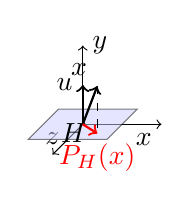
\begin{tikzpicture}

    % Axes
    \draw[->] (0,0,0) -- (1,0,0) node[anchor=north east]{$x$};
    \draw[->] (0,0,0) -- (0,1,0) node[anchor=west]{$y$};
    \draw[->] (0,0,0) -- (0,0,1) node[anchor=south]{$z$};

    % Hyperplan H dans le plan xz
    \filldraw[fill=blue!20,opacity=0.5] (-0.5,0,-0.5) -- (0.5,0,-0.5) -- (0.5,0,0.5) -- (-0.5,0,0.5) -- cycle;
    \node at (0,0,0.3) {$H$};

    % Vecteur u normal à H, orienté le long de l'axe y
    \draw[->,thick] (0,0,0) -- (0,0.5,0) node[anchor=east]{$u$};

    % Vecteur x dans E
    \draw[->,thick] (0,0,0) -- (0.3,0.6,0.3) node[anchor=south east]{$x$};

    % Projection PH(x) sur H
    \draw[dashed] (0.3,0.6,0.3) -- (0.3,0,0.3);
    \draw[->,thick,red] (0,0,0) -- (0.3,0,0.3) node[anchor=north]{$P_{H}(x)$};

\end{tikzpicture}
\end{center}


\item Deux sous-espaces $F$ et $G$ sont en somme directe si et seulement si \[F \cap G = \{0\}.\]

\item Si $F_1, \ldots, F_r$ sont des sous-espaces de dimension finie de $E$, alors \[\dim\left(\sum_{i=1}^{r} F_i\right) \leq \sum_{i=1}^{r} \dim(F_i)\]avec égalité si et seulement si la somme est directe.

\item Si $u$ et $v$ commutent, alors $\text{Im}(u)$ et $\text{ker}(u)$ sont stables par $v$.

\item Si $\lambda_1, \ldots, \lambda_p$ sont des valeurs propres distinctes de $u$, alors les sous-espaces propres associés $E_{\lambda_1}, \ldots, E_{\lambda_p}$ sont en somme directe.

\item Deux matrices semblables ont le même polynôme caractéristique

\item Le polynôme caractéristique de \(A\) est un polynôme unitaire qui s'écrit \[\chi_A(X) = X^n - \text{tr}(A)X^{n-1} + \cdots + (-1)^n\det(A).\]

\item Les racines du polynôme caractéristique de $A$ (resp. $u$) sont exactement les valeurs propres de $A$ (resp. $u$).

\item Pour tout $\lambda \in \text{Sp}(u)$, on a \[\dim(E_{\lambda}) \leq \text{mult}(\lambda).\]

\item Soit $u \in \mathcal{L}(E)$. Les assertions suivantes sont équivalentes :
\begin{enumerate}
    \item $u$ est diagonalisable.
    \item La somme des sous-espaces propres de $u$ est égale à $E$.
    \item $\sum_{\lambda \in \text{Sp}(u)} \dim(E_{\lambda}) = \dim(E)$.
\end{enumerate}

\begin{center}
Tout les polynomes caractéristiques sont annulateurs mais pas l'inverse !
\end{center}

\item Un opérateur $u \in \mathcal{L}(E)$ est diagonalisable dans $\mathbb{R}$ ou $\mathbb{C}$ si et seulement si le polynôme caractéristique $\chi_u$ est SDRS.

\item Un opérateur $u \in \mathcal{L}(E)$ est diagonalisable dans $\mathbb{R}$ si et seulement si le polynôme caractéristique $\chi_u$ est SD et si, pour toute valeur propre $\lambda$, on a \[\dim(E_{\lambda}) = \text{mult}(\lambda).\]

\item Un opérateur $u \in \mathcal{L}(E)$ est diagonalisable dans $\mathbb{R}$ ou $\mathbb{C}$ si et seulement un polynôme annulateur est SDRS.

\item Un opérateur $u \in \mathcal{L}(E)$ est TZ dans $\mathbb{R}$ ou $\mathbb{C}$ si et seulement si le polynôme caractéristique $\chi_u$ est SD.

\item Un opérateur $u \in \mathcal{L}(E)$ est diagonalisable dans $\mathbb{R}$ ou $\mathbb{C}$ si et seulement si un polynôme annulateur est SD.

\section*{Méthode}

\subsection*{Diagonaliser effectivement une matrice \( A \)}
\textit{Pour diagonaliser effectivement une matrice \( A \), on procède de la manière suivante :}

\begin{enumerate}
    \item \textit{On cherche ses valeurs propres, par exemple en calculant le polynôme caractéristique.}
    \item \textit{Pour chaque valeur propre, on cherche une base de l'espace propre associé.}
    \item \textit{On a alors \( A = PDP^{-1} \) où \( P \) est la matrice dont les colonnes sont constituées par la réunion des bases des espaces propres, et la matrice \( D \) est la matrice diagonale dont les coefficients sont les valeurs propres de \( A \), écrites dans le même ordre que les vecteurs colonnes de \( P \).}
\end{enumerate}



\item Un endomorphisme de $E$ admettant $n$ valeurs propres distinctes est diagonalisable.

\item Une matrice $A \in M_n(K)$ est diagonalisable si et seulement si $A$ est semblable à une matrice diagonale.

\item Soit $u \in \mathcal{L}(E)$. Les assertions suivantes sont équivalentes :
\begin{enumerate}
    \item $u$ est nilpotent.
    \item Le polynôme caractéristique $\chi_u(X) = X^n$.
    \item Il existe une base de $E$ dans laquelle la matrice de $u$ est triangulaire supérieure avec des zéros sur la diagonale.
\end{enumerate}

\item Une matrice $A \in M_n(K)$ est nilpotente si et seulement si $A$ est semblable à une matrice triangulaire supérieure avec des zéros sur la diagonale.

\item Un projecteur de $E$ est autoadjoint si et seulement si c'est un projecteur orthogonal.


\item Théorème spectral: Soit $u \in \mathcal{L}(E)$. Les propriétés suivantes sont équivalentes :
\begin{enumerate}
    \item $u$ est autoadjoint.
    \item $E$ est la somme directe orthogonale des sous-espaces propres de $u$.
    \item Il existe une base orthonormale de $E$ constituée de vecteurs propres pour $u$.
\end{enumerate}

\item Corollaire du théorème spectral: Soit $M \in M_n(\mathbb{R})$. Alors $M$ est symétrique si et seulement s'il existe une matrice orthogonale $P$ et une matrice diagonale $D$ telle que $M = PDP^T$.

\item Proposition: Soit $u \in \mathcal{S}(E)$. On a les équivalences suivantes :
\begin{itemize}
    \item $u \in \mathcal{S}_+(E) \iff \text{Sp}(u) \subset \mathbb{R}_+$.
    \item $u \in \mathcal{S}_{++}(E) \iff \text{Sp}(u) \subset \mathbb{R}_*^+$.
\end{itemize}

\item 
Soit $u \in \mathcal{L}(E)$. Les assertions suivantes sont équivalentes :
\begin{enumerate}
    \item $u$ est une isométrie vectorielle.
    \item $u$ conserve le produit scalaire : $\forall (x, y) \in E^2, \quad \langle u(x), u(y) \rangle = \langle x, y \rangle$.
    \item $u$ est inversible et $u^{-1} = u^*$.
    \item L'image d'une base orthonormée de $E$ par $u$ est une base orthonormée.
    \item La matrice de $u$ dans une base orthonormée est une matrice orthogonale.
\end{enumerate}

Soit $A \in M_2(\mathbb{R})$. Alors :
\begin{itemize}
    \item $A \in SO_2(\mathbb{R})$ si et seulement s'il existe $\theta \in \mathbb{R}$ tel que\[A = \begin{pmatrix}\cos(\theta) & -\sin(\theta) \\\sin(\theta) & \cos(\theta)\end{pmatrix}. \]  \item $A \in O_2(\mathbb{R}) \setminus SO_2(\mathbb{R})$ si et seulement s'il existe $\theta \in \mathbb{R}$ tel que \[A = \begin{pmatrix}
 \cos(\theta) & \sin(\theta) \\
    \sin(\theta) & -\cos(\theta)
    \end{pmatrix}.
    \]
\end{itemize}

\item Soit $E$ un espace euclidien orienté de dimension $3$ et $u \in SO(E)$. Il existe une base orthonormée directe $B$ de $E$ telle que
\[
\text{Mat}_B(u) = \begin{pmatrix}
1 & 0 & 0 \\
0 & \cos(\theta) & -\sin(\theta) \\
0 & \sin(\theta) & \cos(\theta)
\end{pmatrix}.
\]
En particulier, il existe une droite $D$ et un plan $P$ orthogonal à $D$ tel que $u|_D = \text{Id}_D$ et $u|_P$ est une rotation d'angle $\theta$. On dit alors que $u$ est la rotation d'axe $D$ et d'angle $\theta$.










\end{itemize}

\subsection{Caractérisations sur l'inversibilité d'une matrice}
A \( \in M_{n,p}(K) \) (par défaut) est inversible \underline{SI ET SEULEMENT SI} : 
\begin{itemize}[label=$\ast$]
	\item A est de determinant non nul
	\item 0 n'est pas valeur propre de A
	\item Ker(A)= \{0\}
	\item Il existe un polynôme annulateur de A dont 0 n'est pas racine
	\item ses coefficients diagonaux sont tous non nuls dans le cas d'une matrice triangulaire (et son inverse est elle aussi triangulaire supérieure)
	\item \(rg(A) = n\) si \(A \in M_n(K)\)
	\item \( \forall X \in K^n\) \(AX=0 \rightarrow X=0\) si \( A \in M_n(K) \) 
	\item \(\exists B \in M_n(K), AB = I_n\), alors \(A \in M_n(K)\) et B sont inversibles et inverse l'une de l'autre
\end{itemize}

\subsection{Propriété sur la semblablilité de deux matrices}
A et B sont semblables \underline{SI ET SEULEMENT SI} : 
\begin{itemize}[label=$\ast$]
	\item \( det(A) = det(B) \)
	\item \( tr(A) = tr(B) \)
	\item \( rg(A) = rg(B) \)
\end{itemize}

\subsection{Propriété sur la diagonalisation de matrice}
\begin{itemize}[label=$\ast$]
	\item Si le polynôme caractéristique de u est scindé à racines simples, alors u est diagonalisable
	\item A est diagonalisable \underline{si et seulement si} elle est symétrique réelle
\end{itemize}


\subsection{Formules à connaitre}
\begin{itemize}[label=$\ast$]
	\item \textbf{Formule du binôme pour les matrices :} Si \( A, B \in M_n(K) \) sont telles que \( AB = BA \), alors \[ (A + B)^n = \sum_{k=0}^{n} \binom{n}{k} A^k B^{n-k} \].

\end{itemize}

\subsection{Propriété sur les dimensions}
\begin{itemize}[label=$\ast$]
	\item \( dim(E \times F) = dim(E) + dim(F) \)
	\item \( dim(E \oplus F) = dim(E) + dim(F) \)
	\item \( dim(F + G) = dim(F) + dim(G) - dim(F \cap G) \)
	\item \(dim L(E,F) = dim(E) \times dim(F) \)
	\item \underline{Théorème du rang} : dim(E)  = rg(u) + dim(Ker u)
	\item dim(Ker A) + rg(A) = p avec \(A \in M_{n,p}(K)\)
\end{itemize}

\subsection{Propriété sur la liberté d'une famille}
\begin{itemize}[label=$\ast$]
	\item Toutes sous-famille d'une famille finie liée est liée
	\item Une famille finie de polynômes non nuls de degrés 2 à 2 distincts est libre
	\item Toutes sous-famille d'une famille finie libre est libre
	\item  Toutes famille de vecteurs propres associées à des valeurs propres deux à deux distinctes est libre
	\item \( (x,y) \) liée signifie que \( x \) et \( y \) sont colinéaires.
\end{itemize}

\subsection{Propriété sur le rang d'une matrice}
\begin{itemize}[label=$\ast$]
	\item la trace d'un projecteur est égal à son rang
	\item Une matrice et sa transposée ont même rang
	\item Une matrice est de rang r ssi elle est équivalente à la matrice \( J_r \)
	\item Deux matrices de même taille sont équivalentes ssi elles ont même rang
	\item une sous matrice de A a un rang inférieur à A
\end{itemize}

\subsection{Propriété sur la trace d'une matrice}
\begin{itemize}[label=$\ast$]
	\item tr(AB) = tr(BA)
	\item \(tr(v \circ u) = tr(u \circ v) \)
\end{itemize}

\subsection{Propriété sur l'hyperplan}
\begin{itemize}[label=$\ast$]
	\item H hyperplan de E \( \leftrightarrow dim(H) = dim(E)-1 \)
	\item Soit H un SEV de E. Alors H est un hyperplan de E ssi il existe une droite vectorielle D telle que \(E = H \oplus D \)
\end{itemize}

\subsection{Propriété sur l'injectivité, la surjectivité et la bijectivité d'une application}
\begin{itemize}[label=$\ast$]
	\item Une application \(u \in L(E,F) \) est injective ssi \(Ker(u) = \{0\} \)
	\item Soit E et F deux EV de même dimensions finie. On a que \(u \in L(E,F) \) on a :  u surjective \( \Leftrightarrow \) u injective \( \Leftrightarrow \) u bijective
\end{itemize}

\subsection{Propriété sur les valeurs propres, vecteurs propres et les sous espaces propres}
\begin{itemize}[label=$\ast$]
	\item Un scalaire \( \lambda \in K \) est une valeur propre de A ssi il est racine du polynôme caractéristique de A
	\item Si deux endomorphismes commutent, les sous espaces propres de l'un sont stable par l'autre
	\item Si A est une matrice triangulaire, alors l'ensemble de ses valeurs propres est sa diagonale
	\item Deux matrices semblambles ont le même spectre et les sous-espaces propres associés sont de même dimension
	\item on a pour tout \( \lambda \in Sp(u) \) : \( 1 \leq dim(E_{\lambda}(u) \leq m(\lambda) \)
	\item \underline{Théorème de Cayley-Hamilton} : Le polynôme caractéristique de u annule u
	\item Si \( (\lambda_i)_{i \in I} \) est une famille finie de valeurs propres de u deux à deux distinctes, alors les sous espaces propres associées \(E_{\lambda_{i}}(u)\) , pour \(i \in I \) , sont en somme directe.
\end{itemize}

\subsection{Propriété sur les EV de dimension fini}

\section{Analyse}

\subsection{Propriétés non triées encore}

\begin{itemize}[label=$\ast$]
	\item \( \sum_{k=1}^{n}k = \frac{n(n+1)}{2} \)
	\item \underline{Somme des termes d'une suite arithmétique} : Soit \( (u_k)_{k \in N} \) une suite arithmétique. Alors pour \( (p,n) \in N^2 \) tel que \( p \leq n \), : \(  \sum_{k=p}^{n}u_k = (n-p+1) \frac{u_p + u_n}{2} \)
	\item Pour \(n \in N \) : \( \sum_{k=1}^n k^2 = \frac{n(n+1)(2n+1)}{6} \)
	\item \underline{Somme des termes d'une suite géométrique} : Soit \((u_n)_{n \in N} \) une suite géométrique de raison \( a \neq 1\). Alors \( \forall (p,n) \in N^2 \) tel que \(p \leq n \) : \( \sum_{n=p}^n u_k = \frac{u_p - u_{n+1}}{1-a} \)
	\item \underline{Relation de Pascal} : \( \forall{(n,p) \in N* \times Z} : \binom{n}{p} = \binom{n-1}{p} + \binom{n-1}{p-1} \)
	\item \underline{Symétrie du coefficient binomial} : \( \forall{(n,p) \in N \times Z} : \binom{n}{p} = \binom{n}{n-p} \)
	\item \underline{Formule du binôme de Newton} : soit \((a,b) \in R^2\) et \(n \in N\) : \((a+b)^n = \sum_{p=0}n \binom{n}{p}a^p b^{n-p} \)
	\item Toute partie non vide et majorée (resp. minorée) de R possède une borne supérieure (resp. inférieure)
	\item \underline{Caractérisation de la borne supérieure} : Soit A une partie de R et \(a \in R \). Alors on a a = Sup(A) \underline{si, et seulement si} : \( \forall x \in A, x \leq a\) et \( \forall b<a, \exists x \in A, b<x \)
	\item \underline{Théorème des suites adjacentes} : Si deux suites sont adjacentes, alors elles convergent vers une limite commune
	\item \underline{Théorème de Bolzano Weierstrass} : Toute suite bornée possède au moins une sous-suite convergente
 	\item Une partei A de R est dense dans R, \underline{si, et seulement si}, pour tout réel x, on peut trouver une suite d'éléments de A qui convergent vers x
	\item L'ensemble des suites bornées est stable par somme et par produit
	\item Toute suite convergente est bornée
	\item \textbf{Fonction \( k \)-lipschitzienne} : Soit \( f: I \to R \) une fonction et \( k \in R^+ \). Alors \( f \) est \( k \)-lipschitzienne si et seulement si pour tout \( x, y \in I \), on a : \( |f(x) - f(y)| \leq k |x - y| \).
	\item \underline{Formule d'intégration par parties} : \( \forall u, v \in C^1(\mathcal{I}), \quad \int u \, dv = uv - \int v \, du \)
	\item \underline{Formule de Taylor avec reste intégrale} : \( f(x) = \sum_{k=0}^{n} \frac{f^{(k)}(a)}{k!}(x-a)^k + \int_{a}^{x} \frac{f^{(n+1)}(t)}{(n)!}(x-t)^{n} \, dt \)
	\item \underline{inégalité de Taylor Lagrange} : 
	\item \textbf{Limite en un point :} Soit \( f: I \rightarrow R \) une fonction, \( a \) un point de \( I \) ou une extrémité de \( I \), et \( \ell \in R \). On dit que \( f \) admet pour limite \( \ell \) en \( a \) si pour tout \( \epsilon > 0 \), il existe \( \eta > 0 \) tel que pour tout \( x \in I \) avec \( |x - a| < \eta \), on a \( |f(x) - \ell| < \epsilon \).

	\item \textbf{Limite en \( +\infty \) :} Soit \( f: I \rightarrow R \) une fonction, \( a \) une extrémité de \( I \). On dit que \( f \) admet pour limite \( +\infty \) en \( a \) si pour tout \( M > 0 \), il existe \( \eta > 0 \) tel que pour tout \( x \in I \) avec \( |x - a| < \eta \), on a \( f(x) > M \).

	\item \textbf{Limite en \( +\infty \) :} Soit \( f: [a, +\infty[ \rightarrow R \) et \( \ell \in R \). On dit que \( f \) admet pour limite \( \ell \) en \( +\infty \) si pour tout \( \epsilon > 0 \), il existe \( A > 0 \) tel que pour tout \( x \in [a, +\infty[ \) avec \( x \geq A \), on a \( |f(x) - \ell| < \epsilon \).

	\item \textbf{Limite en \( +\infty \) :} Soit \( f: [a, +\infty[ \rightarrow R \). On dit que \( f \) admet pour limite \( +\infty \) en \( +\infty \) si pour tout \( M > 0 \), il existe \( A > 0 \) tel que pour tout \( x \in [a, +\infty[ \) avec \( x \geq A \), on a \( f(x) > M \).

	\item \textbf{Théorème (caractérisation séquentielle de la limite) :} 
Une fonction \( f \) admet pour limite \( \ell \) en \( a \) si et seulement si, pour toute suite \( (x_n) \) qui converge vers \( a \), la suite \( (f(x_n)) \) converge vers \( \ell \).

	\item Si une fonction est dérivable en un point, alors elle est continue en ce point

	\item \textbf{Théorème de Rolle :} Soit \( f : [a, b] \rightarrow R \) une fonction continue sur \([a, b]\), dérivable sur \((a, b)\) et telle que \(f(a) = f(b)\). Alors il existe \(c\) appartenant à \((a, b)\) tel que \(f'(c) = 0\).

	\item \textbf{Théorème des accroissements finis :} Soit \( f : [a, b] \rightarrow R \) une fonction continue sur \([a, b]\) et dérivable sur \((a, b)\). Alors il existe \( c \) appartenant à \((a, b)\) tel que
\[ f(b) - f(a) = f'(c)(b - a) \].

	\item \textbf{Inégalité des accroissements finis :} Soit \( f : [a, b] \rightarrow R \) une fonction continue sur \([a, b]\) et dérivable sur \((a, b)\). Supposons qu'il existe \( M > 0 \) tel que, pour tout \( t \in ]a, b[ \), \( |f'(t)| \leq M \). Alors :
\[ |f(b) - f(a)| \leq M|b - a| \].

	\item \textbf{Formule de Leibniz :} Soient \( f \) et \( g \) deux fonctions \( n \) fois dérivables sur \( I \). Alors \( fg \) est \( n \) fois dérivable sur \( I \) et
\[ (fg)^{(n)} = \sum_{k=0}^{n} \binom{n}{k} f^{(n-k)}g^{(k)} \].

	\item \textbf{Définition de la convexité :} Une fonction \( f \) est dite convexe si, pour tous \( x, y \in I \) et tout \( \lambda \in [0, 1] \), on a
\[ f(\lambda x + (1-\lambda)y) \leq \lambda f(x) + (1-\lambda)f(y) \].

	\item \textbf{Théorème (inégalité des pentes) :} Soit \( f : I \rightarrow R \). Les assertions suivantes sont équivalentes :
1. \( f \) est convexe sur \( I \).
2. Pour tout \( a \in I \), la fonction \( x \mapsto f(x) - f(a)(x - a) \) est croissante sur \( I \setminus \{a\} \).
3. Pour tous \( a, b, c \in I \) avec \( a < b < c \), on a
   \[ f(b) - f(a) \frac{b - a}{b - c} \leq f(c) - f(a) \frac{c - a}{b - c} \leq f(c) - f(b) \frac{c - b}{b - c}. \]

	\item \textbf{Théorème (inégalité de Jensen) :} Une fonction \( f \) est convexe si et seulement si, pour tout \( n \geq 2 \), pour tous \( x_1, \ldots, x_n \in I \) et pour tous les réels \( \lambda_1, \ldots, \lambda_n \) de \( [0, 1] \) tels que \( \sum_{i=1}^{n} \lambda_i = 1 \), alors
\[ f\left(\sum_{i=1}^{n} \lambda_i x_i\right) \leq \sum_{i=1}^{n} \lambda_i f(x_i) \].





\end{itemize}


\section{Probabilité}
	
Soient \( E \) et \( F \) deux ensembles finis. Alors

\begin{itemize}
	\item Si \( E \subseteq F \), on a \( \text{card}(E) \leq \text{card}(F) \), avec égalité si et seulement si \( E = F \).
	\item \( \text{card}(E \times F) = \text{card}(E) \times \text{card}(F) \).
	\item \( \text{card}(E \cup F) = \text{card}(E) + \text{card}(F) - \text{card}(E \cap F) \).
	\item Le cardinal des applications de \( E \) dans \( F \) vaut \( (\text{card} \, F)^{\text{card}(E)} \).
	\item \( \text{card}(\mathcal{P}(E)) = 2^{\text{card}(E)} \).
	\item $P(\emptyset) = 0;$
	\item Pour tout $A \in \mathcal{P}(\Omega)$, $P(\overline{A}) = 1 - P(A);$
	\item Pour tous $A, B \in \mathcal{P}(\Omega)$, $A \subset B \Rightarrow P(A) \leq P(B);$
 	\item Pour tous $A, B \in \mathcal{P}(\Omega)$, $P(A \cup B) = P(A) + P(B) - P(A \cap B);$
	\item Pour toute famille $A_1, \ldots, A_p$ d'événements deux à deux incompatibles, $P(A_1 \cup \cdots \cup A_p) = P(A_1) + \cdots + P(A_p);$
	\item Pour tout système complet d'événements $A_1, \ldots, A_p$, $P(A_1 \cup \cdots \cup A_p) = 1.$
	\item Si \( A_1, \ldots, A_n \) sont des événements mutuellement indépendants, et si pour chaque \( i \in \{1, \ldots, n\} \), on pose \( B_i = A_i \) ou \( B_i = \overline{A_i} \), alors les événements \( B_1, \ldots, B_n \) sont mutuellement indépendants.
	\item \textbf{Proposition :} Si \( B \) est un événement tel que \( P(B) > 0 \), alors \( P_B \) est une probabilité sur \( \Omega \).

	\item \textbf{Formule des probabilités composées :} Soit \( A_1, \ldots, A_m \) des événements tels que \( P(A_1 \cap \cdots \cap A_{m-1}) \neq 0 \). Alors : \[ P(A_1 \cap \cdots \cap A_m) = P(A_1) P(A_2 | A_1) P(A_3 | A_1 \cap A_2) \cdots P(A_m | A_1 \cap \cdots \cap A_{m-1}) \].
	\item \textbf{Formule des probabilités totales :} Soit \( A_1, \ldots, A_n \) un système complet d'événements, tous de probabilité non nulle. Soit \( B \) un événement. Alors :
\[ P(B) = \sum_{i=1}^{n} P(A_i) P(B | A_i) \].
	\item \textbf{Formule de Bayes pour deux événements :} Si \( A \) et \( B \) sont deux événements de probabilité non nulle, alors
\[ P(A | B) = \frac{P(B | A) P(A)}{P(B)} \].
	\item \textbf{Proposition :} Si \( B \) est un événement tel que \( P(B) > 0 \), alors \( P_B \) est une probabilité sur \( \Omega \).
	\item \textbf{Formule des probabilités composées :} Soit \( A_1, \ldots, A_m \) des événements tels que \( P(A_1 \cap \cdots \cap A_{m-1}) \neq 0 \). Alors :
\[ P(A_1 \cap \cdots \cap A_m) = P(A_1) P(A_2 | A_1) P(A_3 | A_1 \cap A_2) \cdots P(A_m | A_1 \cap \cdots \cap A_{m-1}) \].

	\item \textbf{Formule des probabilités totales :} Soit \( A_1, \ldots, A_n \) un système complet d'événements, tous de probabilité non nulle. Soit \( B \) un événement. Alors :
\[ P(B) = \sum_{i=1}^{n} P(A_i) P(B | A_i) \].

	\item Si \( X \) et \( Y \) sont indépendantes, alors \( E(XY) = E(X) E(Y) \).
    \item \( V(X) = E(X^2) - E(X)^2 \);
    \item \( V(aX + b) = a^2 V(X) \).




\textbf{Propriétés des probabilités :}
\begin{enumerate}
    \item \( P(\emptyset) = 0 \);
    \item Pour tout \( A \in \mathcal{P}(\Omega) \), \( P(\overline{A}) = 1 - P(A) \);
    \item Pour tous \( A, B \in \mathcal{P}(\Omega) \), \( A \subseteq B \implies P(A) \leq P(B) \);
    \item Pour tous \( A, B \in \mathcal{P}(\Omega) \), \( P(A \cup B) = P(A) + P(B) - P(A \cap B) \);
    \item Pour toute famille \( A_1, \ldots, A_p \) d'événements deux à deux incompatibles, 
          \( P(A_1 \cup \cdots \cup A_p) = P(A_1) + \cdots + P(A_p) \);
    \item Pour tout système complet d'événements \( A_1, \ldots, A_p \), \( P(A_1 \cup \cdots \cup A_p) = 1 \).
	\item \textbf{Inégalité de Bienaymé-Tchebychev :} Soit \( X \) une variable aléatoire réelle et soit \( \epsilon > 0 \). Alors 
\[ P(|X - E(X)| \geq \epsilon) \leq \frac{V(X)}{\epsilon^2} \].
	\item \textbf{Inégalité de Markov :} Soit \( X \) une variable aléatoire réelle et soit \( t > 0 \). Alors
\[ P(|X| \geq t) \leq \frac{|E(X)|}{t} \].

\end{enumerate}



\end{itemize}




\end{document}